\documentclass[conference, a4paper]{IEEEtran}
%\IEEEoverridecommandlockouts
% The preceding line is only needed to identify funding in the first footnote
% . If that is unneeded, please comment it
% out.
%\usepackage{cite}
\usepackage{nicefrac}
\usepackage{amsmath,amssymb,amsfonts}
\usepackage[spanish, english]{babel}
\usepackage{algorithmic}
\usepackage{graphicx}
\usepackage{textcomp}
\usepackage[T1]{fontenc}
\usepackage{xcolor}
\usepackage[numbers]{natbib}
\usepackage[]{hyperref}
\usepackage{color}
\usepackage{stringstrings}
\usepackage{xstring, xifthen}
\usepackage{flushend}
\usepackage{stfloats}
\usepackage{siunitx}
\usepackage{tabularx}
\usepackage{fp}
\usepackage[left=1.57cm,right=1.57cm,top=0.95cm,bottom=2.54cm]{geometry}
\usepackage{booktabs}
\newcommand{\BibTeX}{{\rm B\kern-.05em{\sc i\kern-.025em b}\kern-.08em
T\kern-.1667em\lower.7ex\hbox{E}\kern-.125emX}}




\makeatletter
\newcount\my@repeat@count
\newcommand{\myrepeat}[2]{%
    \begingroup
    \my@repeat@count=\z@
    \@whilenum\my@repeat@count<#1\do{#2\advance\my@repeat@count\@ne}%
    \endgroup
}

\makeatother

\makeatletter

\makeatletter
\newcounter{hideCounter}
\newcommand\hidex[1]{%
    \def\mystring{#1}
    \StrLen{\mystring}[\mystringlen]
%\myrepeat{\mystringlen}{x}
    \mystring

}
\makeatother

\newcommand{\espoleta}{ESPOLETA Tecnologías S.R.L.}
\newcommand{\client}{UNNAME~}

\begin{document}
\title{
	Desarrollo del software de la primera estación meteorológica de origen cubano.
	Su uso en el análisis de los efectos del cambio climático en la industria agrícola.
}

\author{\IEEEauthorblockN{\hidex{Lázaro Andrés O'Farrill Nuñez}}
	\IEEEauthorblockA{\textit{\hidex{Estudiante de pregrado de ingeniería
				biomédica}} \\
		\textit{\hidex{Universidad Tecnológica de la Habana ``José Antonio Echeverría'' CUJAE}}\\
		\hidex{https://orcid.org/0000-0002-1146-2775}}\\[1cm]
	Tutores:
	DrC.
	Ivón Oristela Benítez \\ Fac.
	Automática y Biomédica \\ \textit{\hidex{Universidad Tecnológica de la Habana ``José Antonio Echeverría'' CUJAE}}\\ lol@lol.com }

\maketitle

\selectlanguage{spanish} \renewcommand{\tablename}{Tabla} \renewcommand{\arraystretch}{1.5}

\begin{abstract}
	The following work aims to develop the software of the first weather station of Cuban origin, integrating hardware and software that allows capturing and recording meteorological variables such as data on temperature, humidity, atmospheric pressure, etc., in order to analyze and manage data climate change statistics on agricultural processes.

\end{abstract}

\renewcommand{\IEEEkeywordsname}{Palabras Clave}
\begin{IEEEkeywords}
	weather station, climate change, meteorological variables, agricultural processes
\end{IEEEkeywords}

\section{introducción}\label{sec:introduccion}
El cambio climático, afecta a diferentes sectores de la economía, siendo el
sector agrícola uno de los más afectados cada año.
El aumento de las temperaturas termina por reducir la producción de los
cultivos deseados, a la vez que provoca la proliferación de malas hierbas y
pestes.
Los cambios en los regímenes de lluvias aumentan las probabilidades de fracaso
de las cosechas a corto plazo y de reducción de la producción a largo plazo.
Aunque algunos cultivos en ciertas regiones del mundo puedan beneficiarse, en
general se espera que los impactos del cambio climático sean negativos para la
agricultura, amenazando la seguridad alimentaria mundial.
Por estos motivos es necesario realizar estudios estadísticos y realizar
análisis sobre las variables meteorológicas.

Una estación meteorológica, es el lugar donde se realizan mediciones y
observaciones puntuales de los diferentes parámetros meteorológicos utilizando
los instrumentos adecuados para así poder establecer el comportamiento
atmosférico.

El exsecretario general de la Organización Meteorológica afirma: Una estación
meteorológica es el lugar en el que se realizan observaciones del
comportamiento de la atmósfera y del medio ambiente.
La recopilación de datos emitidos por el instrumental meteorológico y su
posterior análisis y estudio permitirán la caracterización espacial y temporal
de los fenómenos atmosféricos, así como la realización de un diagnóstico de la
situación atmosférica en un momento dado.
En función a la estación meteorológica se definen tres parámetros
fundamnetales: humedad, presión atmosférica y temperatura, además de un
conjunto de otras variables meteorólogicas que interactúan entre sí.

\section{fundamentación del proyecto I+D+I}\label{sec:fundamentacion-del-proyecto-i+d+i}

\subsection{Antecedentes}\label{subsec:antecedentes}
El interés de la humanidad por tratar de predecir el clima es prácticamente tan
antiguo como la civilización.
En la época moderna la invención del telégrafo permitió llevar la predicción
del clima a una velocidad nunca antes vista.
A medida que se expandió el telégrafo a través de los Estados Unidos fue creada
una red vigilancia meteorológica sobre su
infraestructura~\cite{ThomasJeffersonTelegraph}.

No fue hasta el siglo XX que los avances en la física atmosférica llevaron a
fundar los sistema de predicción meteorológica numéricos.
En su libro, ``Weather prediction by numerical
process''~\cite{richardsonWeatherPredictionNumerical1922}, Lewis Fry Richardson
señala como pequeñas diferencias en los fluidos atmosféricos pueden ser
ignorados.

Durante la intervención de Estados Unidos en Cuba el Buró de Tiempo de
Washington fabrica en la loma de Casablanca una estación meteorológica
auxiliar.
En 1904 el presidente cubano Tomás Estrada Palma decreta fundar un observatorio
cubano.
Por oposición la plaza de subdirector del observatorio es ocupada por el
Ingeniero Civil, Arquitecto, Dr.
en Ciencias Físicas, Dr. en Ciencias Naturales
y Dr. en Ciencias Marítimas José Carlos Millas Hernández.
Una vez ocupada esta posición creo una red de observadores basada en el
telégrafo.

Este fue el estado de la meteorología hasta 1944, año en que el control del
sistema meteorológico pasa a la marina.
En este período se crean varias nuevas estaciones y con operarios capacitados a
lo largo de Cuba~\cite{cubaHistoriaMeteorologiaCuba}.

\subsection{Estado del arte}\label{subsec:estado-del-arte}
Hay un gran número de compañías desarrollando estaciones meteorológicas.
Sin embargo estas tienen a menudo un elevado coste, o solo son capaces de medir
un número muy limitado de variables.
Los fabricantes de estaciones más populares como Vantage Pro y Libelium tienen
unidades básicas con un coste superior a los siete mil dólares
(\$7,0000)~\cite{botero-valenciaLowCostClimate2022a}.

También hay iniciativas dedicadas a hacer disponibles estaciones automatizadas
de bajo coste y código abierto.
Entre estos proyectos es común encontrar como motivación la necesidad de un
equipo mejor adecuado a las necesidades específicas de una región o individuos
determinados~\cite{bernardesPrototypingLowcostAutomatic2022,
	nettoOpensourceAutomaticWeather2019}.

La relativamente alta popularidad de la que gozan estos equipos recientemente
se debe en gran medida a la amenaza cada vez más real del cambio
climático~\cite{zizingaClimateChangeMaize2022,
	ahmadHistoricalClimateChange2022, taoClimateWarmingOutweighed2022,
	aprakuClimateChangeSmallscale2021}.
A lo largo de todo el mundo las impredecibles variaciones climatológicas
amenazan con provocar una crisis alimentaria nunca antes
vista\cite{ibrahimCombatingClimateChange2022, guoImpactClimateChange2022}.

\subsection{Problema científico}\label{subsec:problema-cientifico}
En muchos de los procesos agrícolas, conocer las variables meteorológicas es de
vital importancia para lograr una mayor efectividad en los procesos, por lo que
es necesario contar con un dispositivo que permita comprobar dichas variables.

Debido al alto coste que conlleva la adquisición de tecnología de punta en el
desarrollo de dispositivos, en búsqueda de la soberanía tecnológica y con el
objetivo de poder dotar al país con tecnologías propias, en el área de la
industria agrícola, la MIPYME \espoleta en colaboración con \client se suma a
estas labores y lleva a cabo el diseño y desarrollo de la primera estación
meteorológica del país.

\subsection{Objeto de estudio}\label{subsec:objeto-de-estudio}
Estación meteorológica Vórtice.

\subsection{Campo de investigación}\label{subsec:campo-de-investigacion}
Estaciones meteorológicas automatizadas.

\subsection{Métodos de investigación}\label{subsec:metodos-de-investigacion}

\subsubsection{Teóricos}
\begin{itemize}
	\item Hipotético-Deductivo: Elaboración de la hipótesis de trabajo a partir de los
	      conocimientos teóricos y experimentales.
	\item Histórico-Lógico: Estudio del comportamiento de aplicaciones de adquisición y
	      análisis de datos para el control de la calidad en la producción de
	      dispositivos.
	\item Analítico-Sintético: Descomposición del problema de investigación en
	      subproblemas de menor complejidad para ser individualmente analizados y
	      solucionados;
	      integrándose, posteriormente a la solución propuesta.
	\item Inductivo-Deductivo: Fundamentación del uso de un sistema automatizado de
	      análisis combinado para el control de la calidad.
\end{itemize}

\subsubsection{Empíricos}
\begin{itemize}
	\item Observación: Observar directamente el equipo para apreciar su estado físico y
	      evaluar los recursos informáticos a la disposición del personal que trabaja en
	      el proyecto.
	\item Experimentación: Desarrollo y análisis de resultados experimentales, utilizando
	      esquemas convencionales y el nuevo sistema propuesto.
\end{itemize}

\subsubsection{Estadísticos}
\begin{itemize}
	\item Para confirmar las estimaciones realizadas en el análisis de los estimadores de
	      exactitud y precisión y comparar el sistema propuesto con los sistemas
	      consultados en las referencias consultadas.
\end{itemize}

\subsection{Hipótesis}\label{subsec:hipotesis}
Si se desarrolla una estación metereológica,con prestaciones similares a otras
estaciones existentes en el mercado internacional, con un costo de producción
no muy elevado, para que de esta forma sea posible ofertar un equipo con buenas
prestaciones técnicas y de seguridad, a un precio competitivo, se contribuirá
al análisis de los efectos del cambio climático sobre los procesos agrícolas.

Si se desarrolla un software para la puesta en marcha y el control de la
calidad de la estación meteorológica, permitirá la comprobación de los
parámetros técnicos del equipo y contribuirá al análisis de los efectos del
cambio climático sobre los procesos agrícolas.

\subsection{Sistema de objetivos}\label{subsec:sistema-de-objetivos}

\subsubsection*{Objetivo general}
Desarrollar el software de la primera estación meteorológica de origen cubano.

\subsubsection*{Objetivos específicos}
Para dar cumplimento al objetivo general, es necesario cumplir con los siguientes objetivos específicos:
\begin{itemize}
	\item Investigar el estado del arte de la estaciones meteorológicas que se ofrecen
	      comercialmente, principales requerimientos técnicos, precios, principales
	      empresas que las desarrollan.
	\item Analizar el hardware (diseño electrónico) del equipo.
	\item Implementar el protocolo de comunicación del dispositivo con la computadora
	      para la transmisión y recepción de datos.
	\item Desarrollar de manera organizada e independiente las funcionalidades
	      propuestas.
	\item Implementar el software del equipo.
\end{itemize}

\subsection{Proyección de tareas}\label{subsec:proyeccion-de-tareas}
En la Figura \ref{fig:gantt}

\begin{figure}[htpb]
	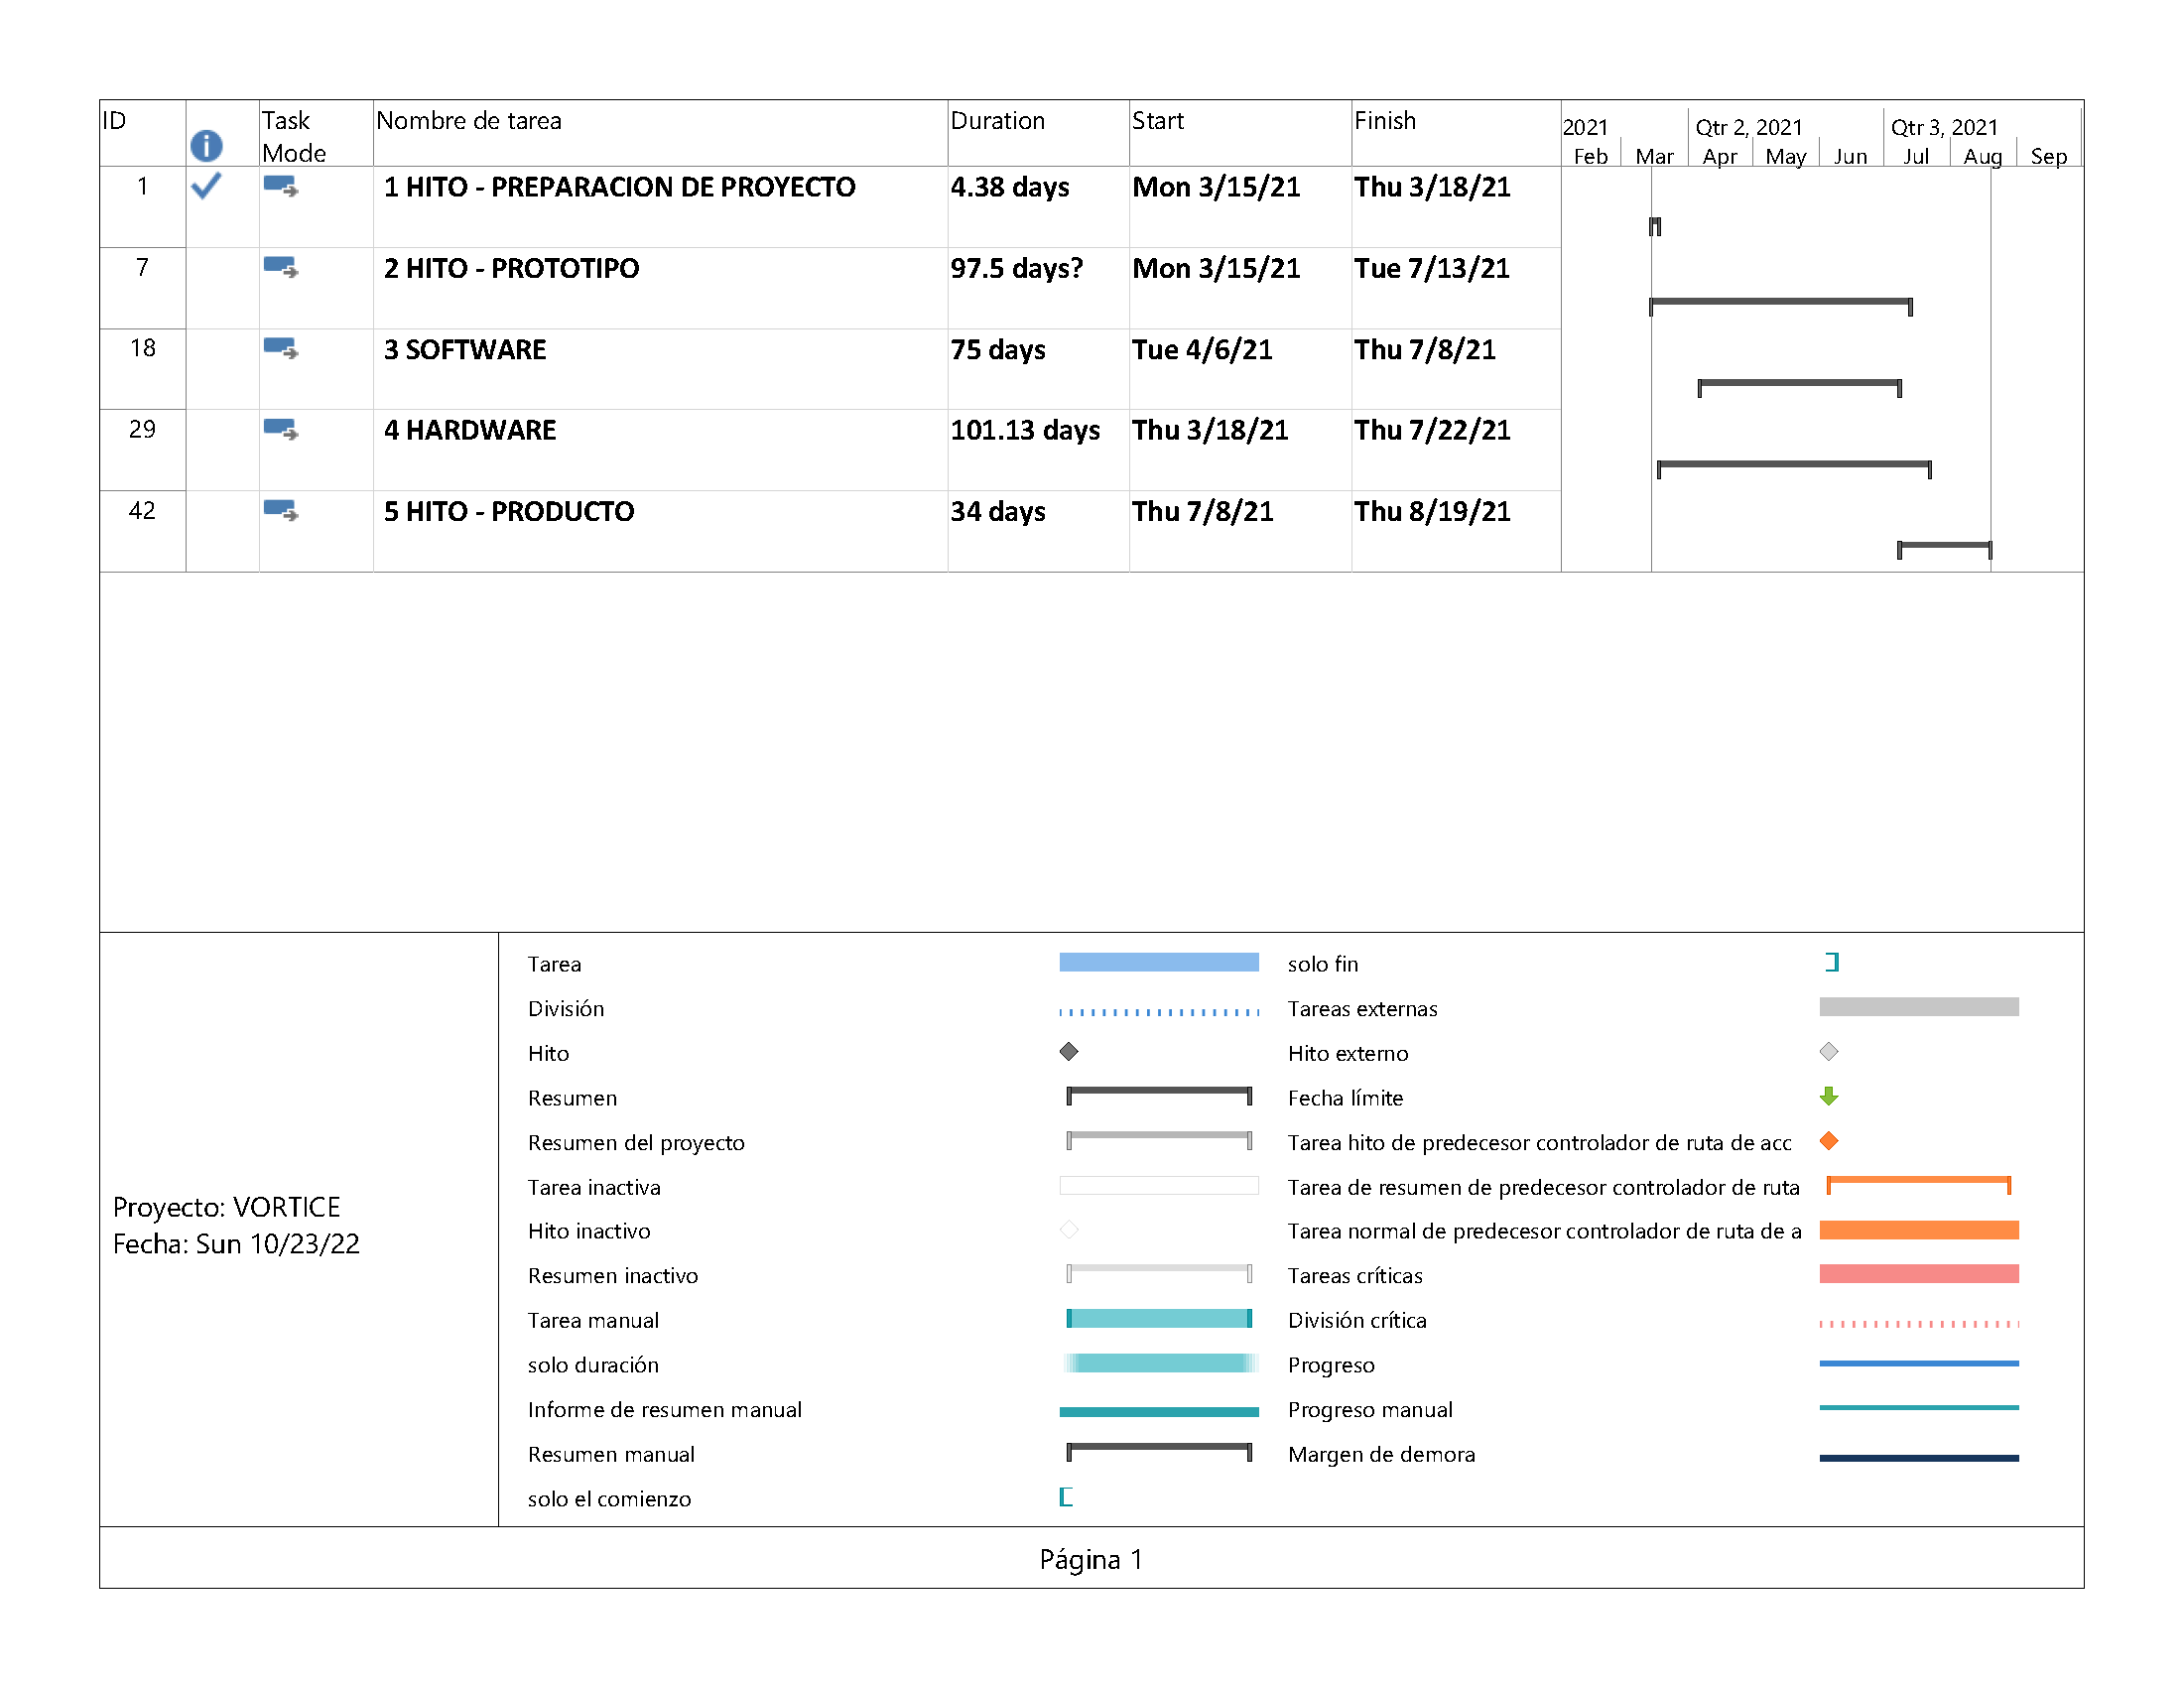
\includegraphics[width=\linewidth]{../shared/figure/gantt} \caption{Proyección de tareas} \label{fig:gantt}
\end{figure}

\section{Factibilidad del proyecto}\label{sec:factibilidad-del-proyecto}

\subsection{Aseguramiento de material}\label{subsec:aseguramiento-de-material} En la sede de la MIPYME \espoleta se encuentran todos los materiales necesarios
para la fabricacición y programación del equipo.

\subsection{Recursos humanos}\label{subsec:recursos-humanos}
El trabajo se realizará durante un período de un año (12 meses).
Para la realización de este proyecto se cuenta con dos tutores los cuales
estarán encargados del asesoramiento de este Trabajo de Diploma y con dos
aspirantes.
La Tabla \ref{tab:salary} presenta los gastos de salario correspondientes a los
participantes, así como los días dedicados por cada uno.
El siguiente análisis corresponde a los meses comprendidos desde enero de 2021
hasta diciembre de 2021.
La forma de calcular los salarios básicos (SB) aparece en \ref{eq:salary}.

\begin{equation}
	\label{eq:salary}
	SB=\sum_i^n A_i * B_i
\end{equation}

donde:

n: Número total de participantes

Ai: Días dedicados a las investigación por participantes.

Bi: Salario diario por participantes (igual al salario mensual dividido por
24).

\begin{table*}[htpb]
	\caption{Gastos por concepto salarial y de seguridad social.}
	\label{tab:salary}
	\begin{tabularx}{\textwidth}{|X X X X X X X|}
		\hline
		trabajador  & sal/mensual & sal/diario & dias/invest.
		            & sal/basico  & sal/comp   & seg/soc                                     \\
		\hline
		Tutor 1     & 6940        & 289.17     & 80           & 23133.33 & 2102.82 & 3533.06 \\
		Tutor 2     & 6940        & 289.17     & 80           & 23133.33 & 2102.82 & 3533.06 \\
		Aspirante 1 & 400         & 16.67      & 120          & 2000     & 181.80  & 305.45  \\
		Aspirante 2 & 400         & 16.67      & 120          & 2000     & 181.80  & 305.45  \\
		\hline
	\end{tabularx}
\end{table*}

\subsection{Recursos materiales}\label{subsec:recursos-materiales}
La Tabla \ref{tab:materials} muestra los recursos materiales empleados y sus
respectivos precios.

\begin{table}[htpb]
	\caption{Gastos por materiales directos}
	\label{tab:materials}
	\begin{tabularx}{\columnwidth}{ |XXXX|}
		\hline
		Dispositivo & Cant & Precio USD & Precio CUP                          \\
		\hline
		Laptop      & 1    & 700        & \FPeval{\result}{clip(700*24)}      %
		\result                                                               \\

		ESP32       & 2    & 3          & \FPeval{\result}{clip(3*24)}\result \\ Arduino Nano & 2 & 2 &
		\FPeval{\result}{clip(2*24)}\result                                   \\ DHT22 & 1 & 0.50 &
		\FPeval{\result}{clip(0.50*24)}\result                                \\ \hline Totales & 4 & 705.50 &
		\FPeval{\result}{clip(16800+72+48+12)}\result                         \\ \hline
	\end{tabularx}
\end{table}

\subsection{Recursos financieros complementarios}\label{subsec:recursos-financieros-complementarios} La Tabla~\ref{tab:finantial_resources} muestra los gastos totales.
%

\begin{table}[htpb]
	\caption{Gastos Totales}
	\label{tab:finantial_resources}
	\begin{tabularx}{\columnwidth}{|XX|}
		\hline
		Gastos Totales & Cant.
		CUP                    \\ \hline OTROS GASTOS & 0 \\ COSTO INDIRECTO & 61009.98 \\ COSTO DIRECTO & 70896.64 \\ COSTO TOTAL (CT) & 131906.62 \\

		\hline
	\end{tabularx}\label{tab:table}

\end{table}

El Salario Complementario \ref{eq:complementary_salary} es 9.09\% del salario
total anual:

\begin{equation}
	\label{eq:complementary_salary} SC=0.0909*SB
\end{equation}

La Seguridad Social \ref{eq:social_security} es 14\% del total de los salarios:

\begin{equation}
	\label{eq:social_security} SS=0.14*(SB+SC)
\end{equation}

Entonces el costo directo de la investigación está dado por
\ref{eq:direct_cost}.

\begin{equation}
	\label{eq:direct_cost}
	CD=SB+SC+SS+MD+DP+OG
\end{equation}

El costo indirecto estimado está dado por \ref{eq:indirect_cost}.
\begin{equation}
	\label{eq:indirect_cost}
	CI=1.4063*SB
\end{equation}

Finalmente el costo total estimado de la investigación está dado por
\ref{eq:total_cost}.
\begin{equation}
	\label{eq:total_cost}
	CT=CD+CI
\end{equation}

\subsection{Alcance de investigación}\label{subsec:alcance-de-investigacion}

\subsubsection*{Científico-técnico} El trabajo de investigación abordará el diseño, desarrollo e implementación de la primera estación meteorológica en nuestro país.

\subsubsection*{Económico}
El costo del proyecto es mucho menor que los encontrados actualmente en la industria meteorológica, la cual se caracteriza por sus prohibitivos precios.
Su desarrollo contribuirá a tener una mayor independencia tecnológica para el sector agrícola.

\bibliographystyle{IEEEtran/bibtex/IEEEtranN}
\bibliography{bibliography}

\end{document}
